\appendix
\chapter{Class diagram} \label{appendix-class}
\begin{figure}[h]
	\begin{center}
		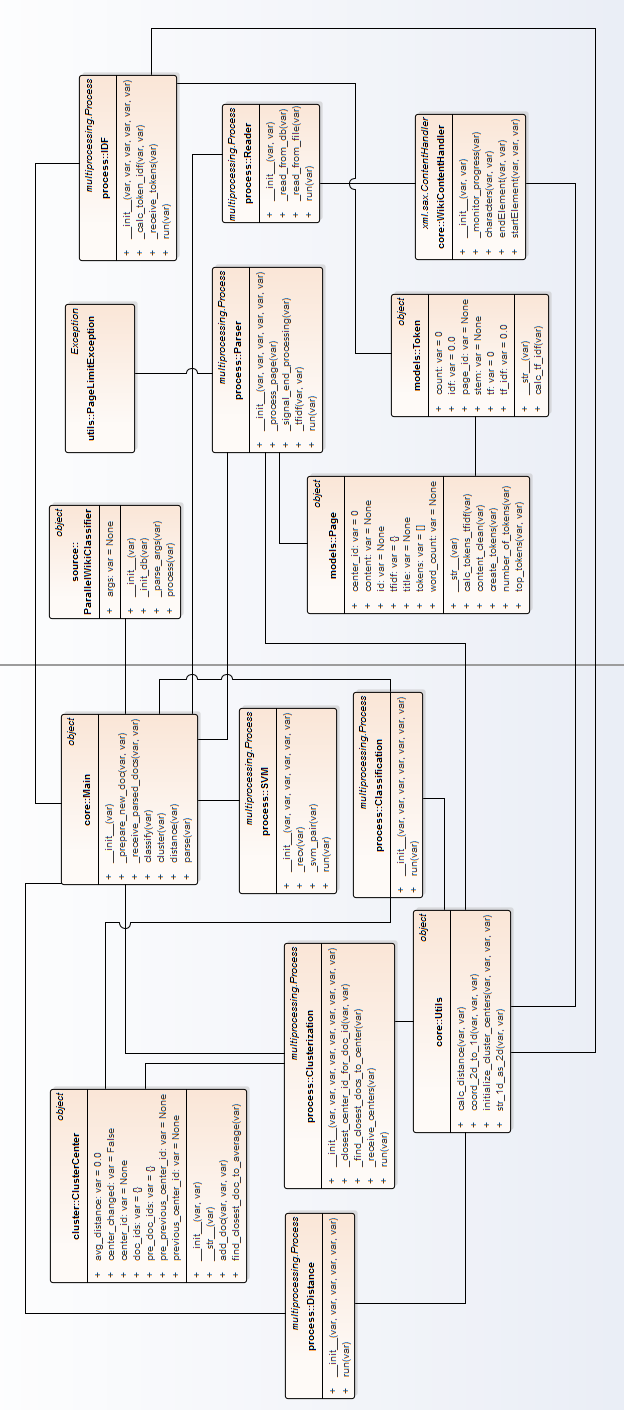
\includegraphics[width=0.72\linewidth]{images/diagrams/class3svm-h.png}
		\label{appendix-class-diagram}
	\end{center}
\end{figure}

\chapter{Sequence diagram} \label{appendix-sequence}
\begin{figure}[h]
	\begin{center}
		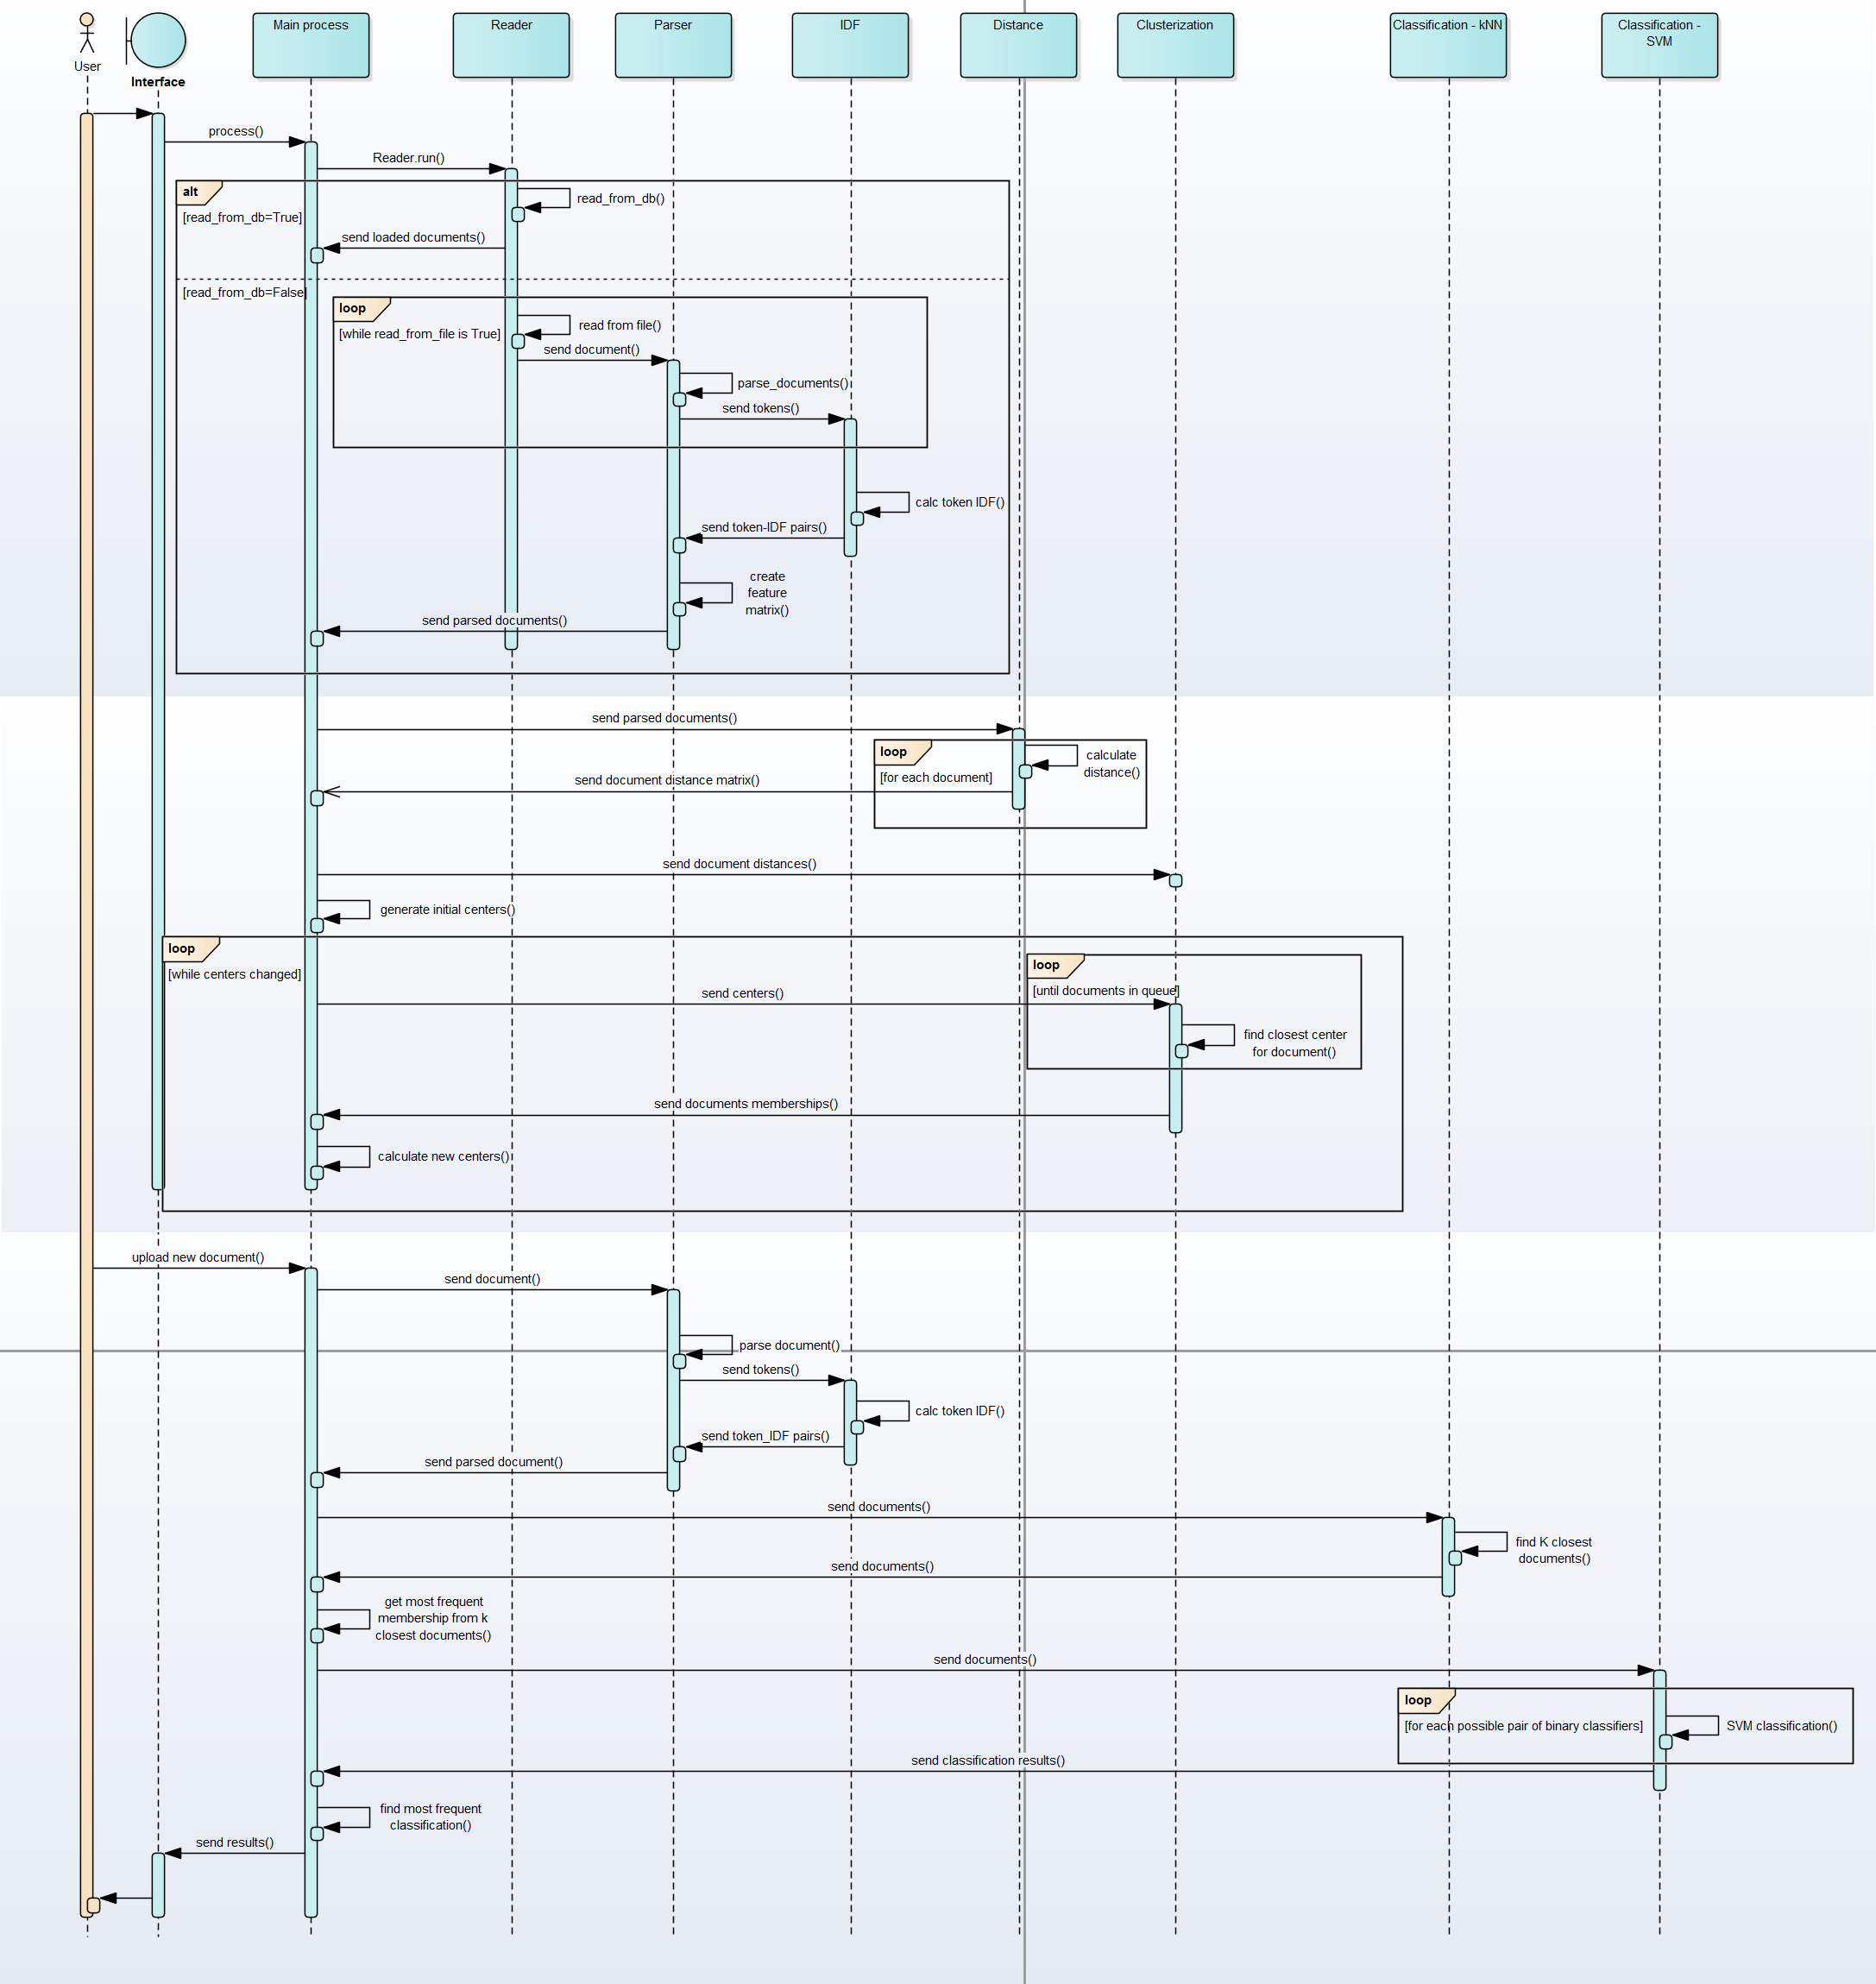
\includegraphics[width=1.2\linewidth]{images/diagrams/seq-full.png}
		\label{appendix-sequence-diagram}
	\end{center}
\end{figure}


\chapter{Instructions}
\section{Installation}
\begin{enumerate}
	\item Install prerequisites: Python 3.5 and git
	\item Clone code repository using command
\begin{lstlisting}[language=Bash, numbers=none]
git clone git@github.com:macsz/parallel-wiki-classifier.git
\end{lstlisting}
	\item To install all required libraries, execute command:
\begin{lstlisting}[language=Bash, numbers=none]
pip install -r source/requirements.txt
\end{lstlisting}
\end{enumerate}
\section{Usage}